\documentclass[bsc,letterpaper,12pt]{csthesis}
%\documentclass[letterpaper,12pt,twoside]{csthesis} % para imprimir de lado y lado


\paperwidth = 21.6cm		% Tamaño de la hoja
\paperheight = 27.9cm

%Margenes horizontales
\hoffset = -2.54cm		% Se elimna el offset horizontal
\oddsidemargin = 4cm
\evensidemargin = 2cm
\textwidth = 15.6cm

%Margenes verticales
\voffset = -2.54cm
\topmargin = 3cm
\headheight = 0cm
\headsep = 0cm
\textheight = 21.9cm
\footskip = 1cm


\usepackage[spanish]{babel}     % Idioma Capitulos y demas
\usepackage[utf8]{inputenc}
\usepackage{lmodern}
\usepackage[T1]{fontenc}
\usepackage{cc/CreativeCommons}  %Licencia

\usepackage{listings} % Ingresar Codigo Fuente
\usepackage{verbatim}
\usepackage{moreverb}
\let\verbatiminput=\verbatimtabinput
\def\verbatimtabsize{8}  % Tabulación en verbatim

% Paquete para el manejo de hipervinculos
\usepackage[b5paper, breaklinks=true, pdfborder={0 0 0},colorlinks=false,pageanchor=true, 
plainpages=false,bookmarksopen=true,bookmarksopenlevel=3, hyperfootnotes=false]{hyperref}

% Paquete para el manejo de tablas
\usepackage{supertabular}

% Paquetes para simbolos
%\usepackage{mathcomp}
\usepackage{latexsym}
\usepackage{pifont}
\usepackage{amsfonts}
\usepackage{amssymb}
\usepackage{wasysym}
\usepackage{colortbl}
\usepackage{multicol} 
\usepackage{booktabs}
\usepackage{multirow}
\usepackage{algorithmic}
\usepackage[Algoritmo]{algorithm}
\usepackage{subfigure}


% Manejo de imagenes PDF y EPS
\newif\ifpdf
\ifx\pdfoutput\undefined
\pdffalse % we are not running PDFLaTeX
\else
\pdfoutput=1 % we are running PDFLaTeX
\pdftrue
\fi

\ifpdf
\usepackage[pdftex]{graphicx}
\else
\usepackage{graphicx}
\fi

\ifpdf
\DeclareGraphicsExtensions{.pdf, .jpg, .tif}
\else
\DeclareGraphicsExtensions{.eps, .jpg}
\fi

% Sangria de comienzo de parrafo
\setlength{\parindent}{0cm}
% Espacio vertical entre dos parrfos
\setlength{\parskip}{0.3cm}

% Definir el nombre de listas
\addto\captionsspanish{%
  \def\prefacename{Prefacio}%
  \def\abstractname{RESUMEN}%
  \def\chaptername{Cap\'{\i}tulo}%
  \def\appendixname{Anexo}%
  \def\listfigurename{Lista de figuras}%
  \def\listtablename{Lista de cuadros}%
  \def\indexname{\'Indice alfab\'etico}%
  \def\figurename{Figura}%
  \def\tablename{Tabla}%
  \def\partname{Parte}%
  \def\enclname{Adjunto}%
  \def\ccname{Copia a}%
  \def\headtoname{A}%
  \def\pagename{P\'agina}%
  \def\seename{v\'ease}%
  \def\alsoname{v\'ease tambi\'en}%
  \def\proofname{Demostraci\'on}%
  \def\glossaryname{Glosario}}
  \addto\captionsspanish{\def\contentsname{CONTENIDO}}
  

%para rotar tablas  
\usepackage{rotating}



%partir palabras
\hyphenation{di-fe-ren-cia pro-pues-to pro-ble-mas po-pu-la-res cons-truccio-nes ne-ce-sa-ria-men-te}

% Inico del documento
\begin{document}
\pagestyle{empty}% Sin número de página
%%% PORTADA

\thispagestyle{empty}
\begin{figure}[!h]
\begin{center}

\includegraphics[scale=0.6]{pictures/udenar.eps}\hspace{1cm}%logo of your university

\includegraphics[scale=0.4]{pictures/sgr.jpg}\hspace{1cm}

\includegraphics[scale=0.9]{pictures/andes.png}
\end{center}
\end{figure}

\vspace{2.5cm}

\begin{center}{\centering \large ANALISIS DE OPORTUNDIDADES ENERGÉTICAS CON FUENTES. ALTERNATIVAS EN EL DEPARTAMENTO DE NARIÑO - ALTERNAR}
\end{center}

\vspace{2.5cm}

\begin{center}{\large Estrategia Biomasa}
\end{center}





\vspace{3.5cm}

\begin{center}{\large OMAR ERNESTO CABRERA ROSERO\\
INGENIERO DE SISTEMAS\\
UNIVERSIDAD DE NARIÑO\\
2015
}
\end{center}



\pagebreak

\newpage
\pagestyle{empty}
\CCbysaInfo	%Licencia  Attribution-ShareAlike 3.0
%\CCbyInfo	%Creative Commons Attribution 3.0
%\CCbyndInfo	%Creative Commons Attribution-No-Derivs 3.0
%\CCbyncInfo	%Creative Commons Attribution-Non-Commercial 3.0
%\CCbyncsaInfo	%Creative Commons Attribution-Non-Commercial-ShareAlike 3.0
%\CCbyncndInfo	%Creative Commons Attribution-Non-Commercial-NoDerivs 3.0


\tableofcontents
\section{Introducción}

\IEEEPARstart Según estudios del Ministerio de Minas y Energía de Colombia, en el departamento de Nariño hay 15 municipios con cobertura eléctrica inferior al 80\% \cite{ministerio_de_minas_y_energia_plan_2008}. Como nueva estratégia para enfrentar esta problemática se ha planteado la medición y estimación de potenciales energéticos en las zonas más viables de la región. Uno de los componentes a analizar es el potencial de biomasa para la generación eléctrica. Sin embargo, uno de los problemas que se plantea para la ubicación de lugares propicios es la ausencia de bases de datos actualizadas en el área de estudio que permitan su respectivo análisis.

Diversas investigaciones han demostrado la utilidad del uso de imágenes satelitales para la generación de modelos que permitan calcular la cantidad de biomasa presente en un determinado lugar. Desde hace más de 30 años, se cuenta con libre acceso al repositorio de imágenes satelitales Landsat \cite{landsat} que con el debido tratamiento pueden ser usadas para calcular valores nominales de biomasa. Sin embargo, dichos modelos requieren la ejecución de trabajo de campo en la zona para inferir fórmulas iniciales a partir de la medición tradicional de una muestra. Dadas las dificultades para realizar dicho trabajo de campo se utilizó imágenes provistas por investigaciones anteriores \cite{baccini2008afirst}, \cite{baccini_estimated_2012} donde se proporciona niveles de biomasa a nivel pan-tropical.  El acceso a imágenes para cada uno de los países tomados en cuenta para el estudio están disponibles en \cite{WHRC}.

Esta investigación esta orientada a cumplir con los requerimientos necesarios para la generación de un modelo de predicción de biomasa y su extrapolación al resto del área de estudio.


El area de estudio de esta investigación fue el departamento de Nariño (Colombia)
el cual esta ubicado en el extremo sur occidental de Colombia, en la frontera con 
Ecuador con una extensión aproximada de 33.268 km, una población de 1,702 millones según
el censo de 2013, su ubicación 
esta en latitud 00° 31' 08'' y 02° 41' 08'' Norte, Longitud 76° 51' 19'' y 79° 01' 34'' Oeste.

\begin{figure}
  \centering
  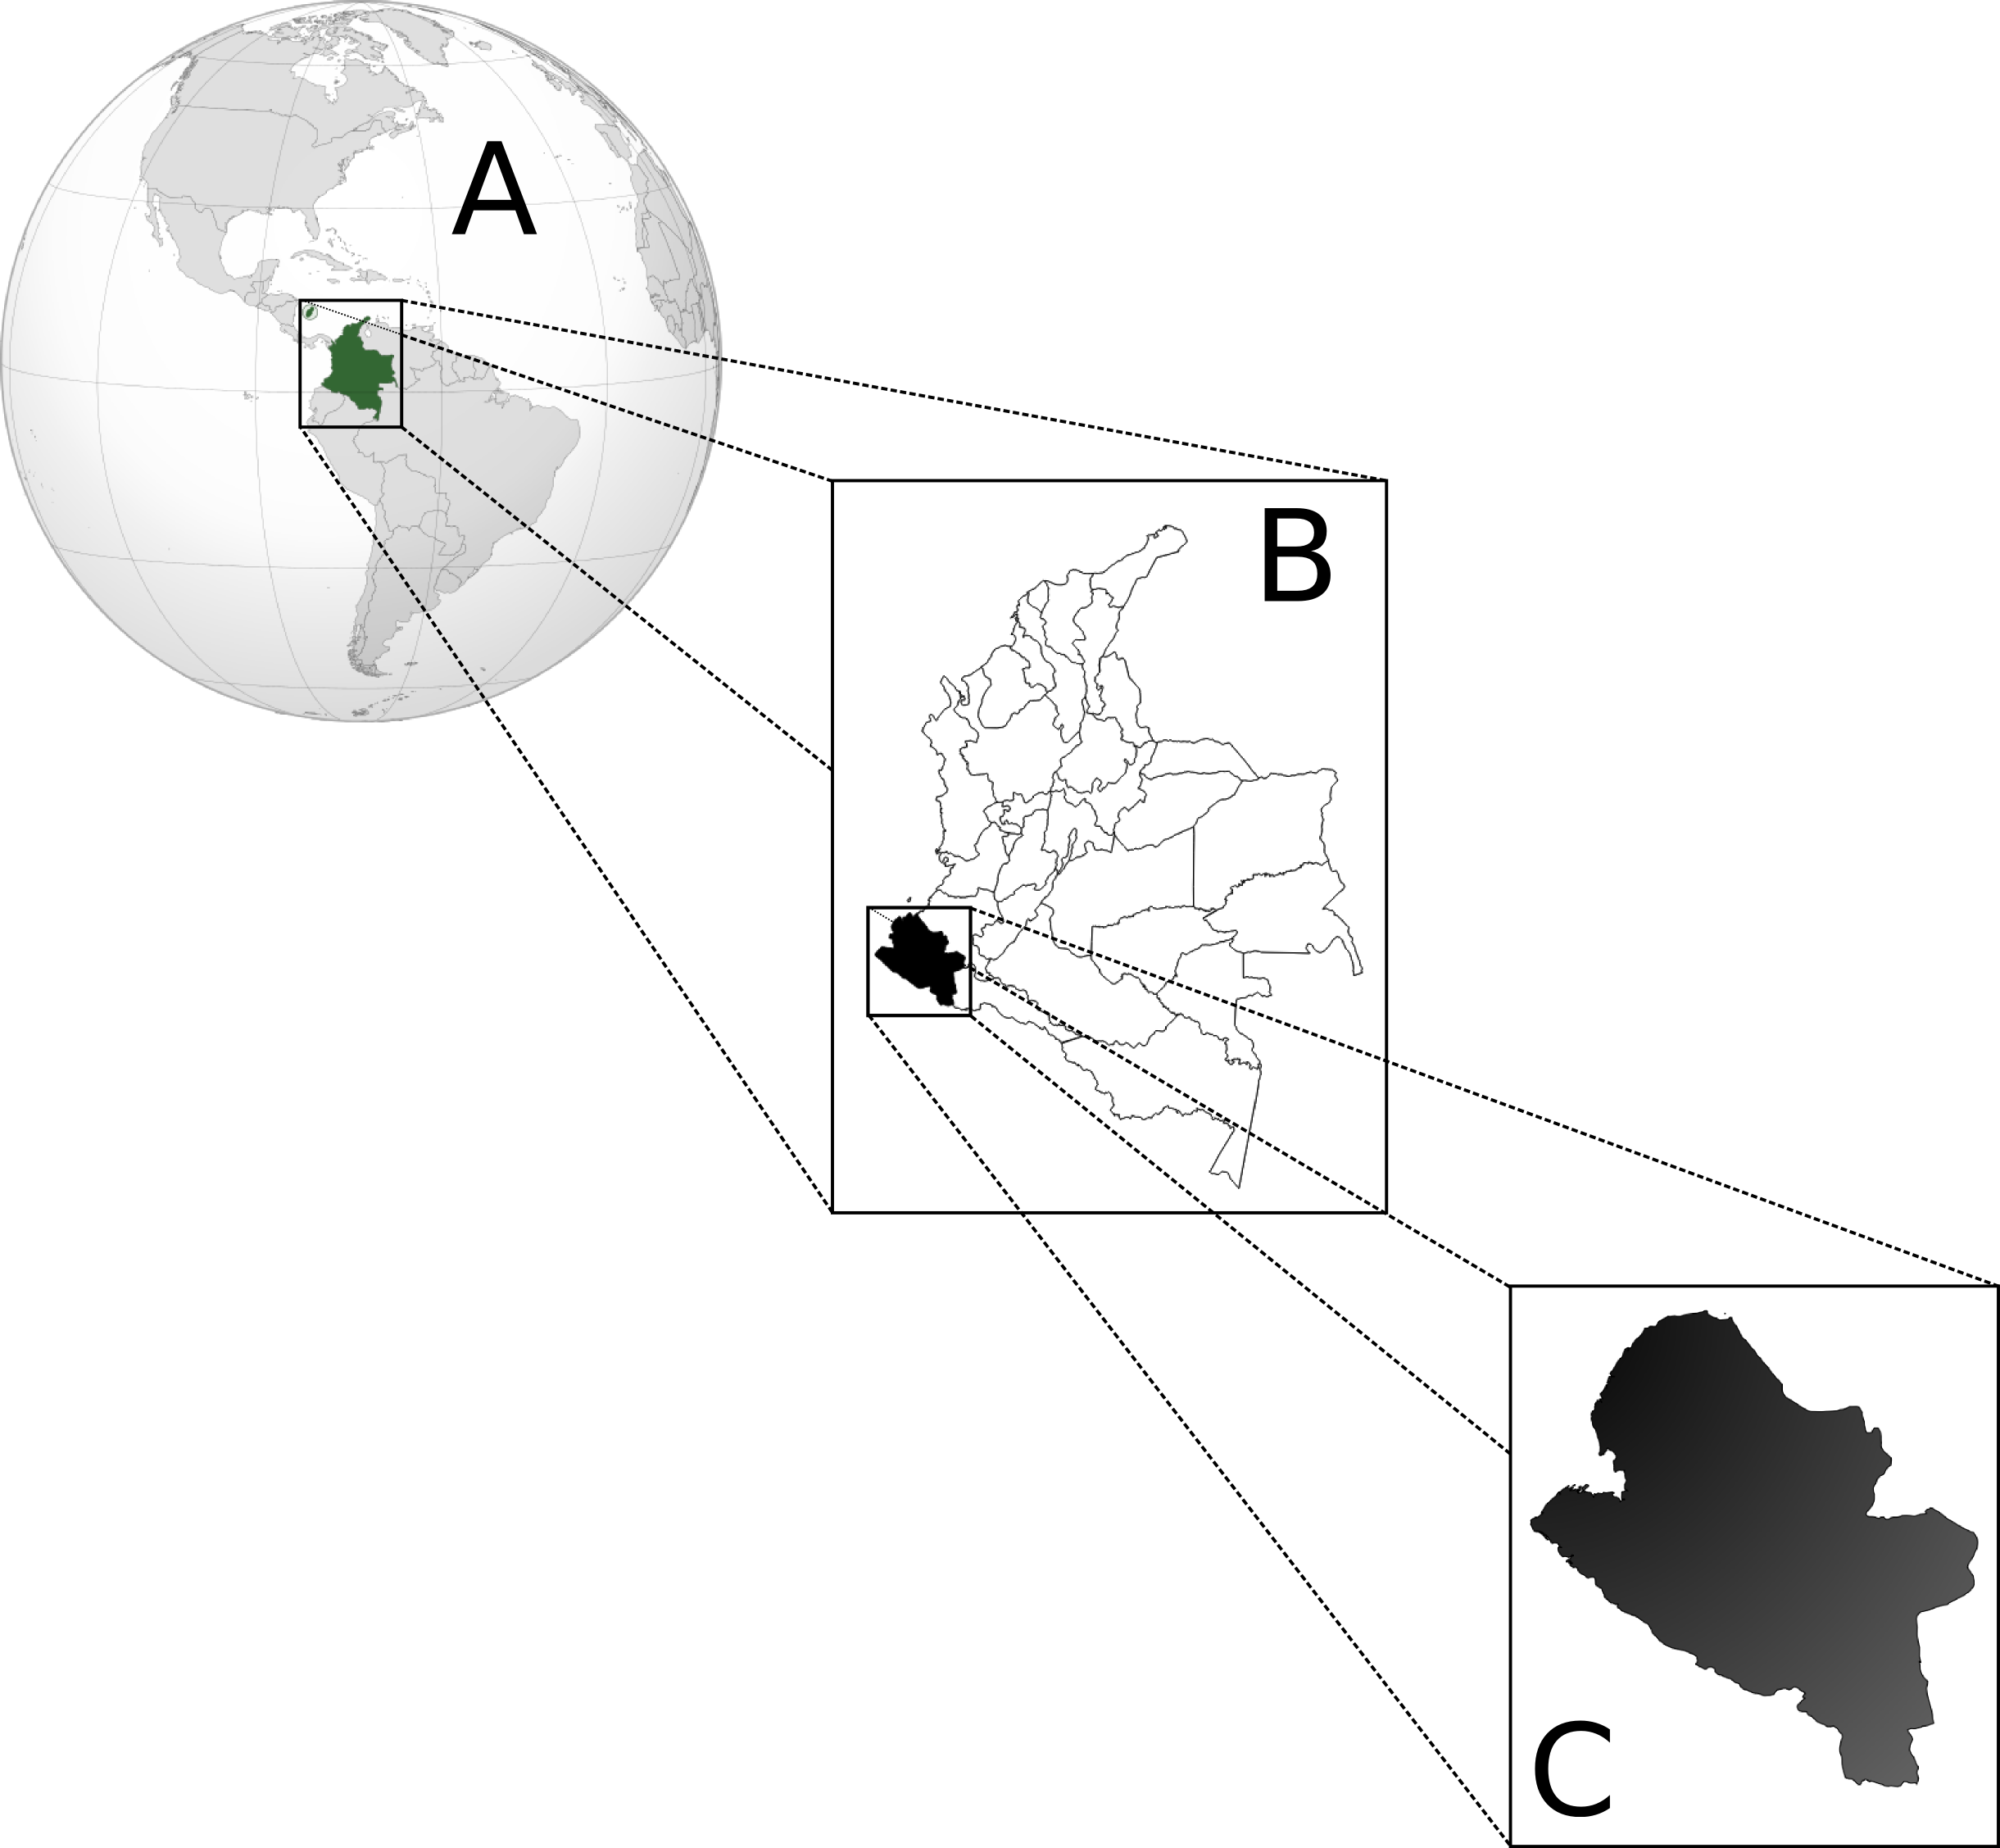
\includegraphics[width = 8cm]{locationNarino.png}
  \caption{Localización area de estudio}
  \label{fig:locationNarino}
\end{figure}
\chapter{Estrategia Biomasa}

Para la recolección de la información de las imágenes satelitales para el departamento de Nariño se descargaron 1362 imagenes del proyecto
Landsat 7, con los path y rows: 009059, 009060, 010058, 010059, 011059, para cubrir todo el departamento de Nariño como lo muestra la figura~\ref{fig:bio1}.

\begin{figure}[!htb]
  \centering
  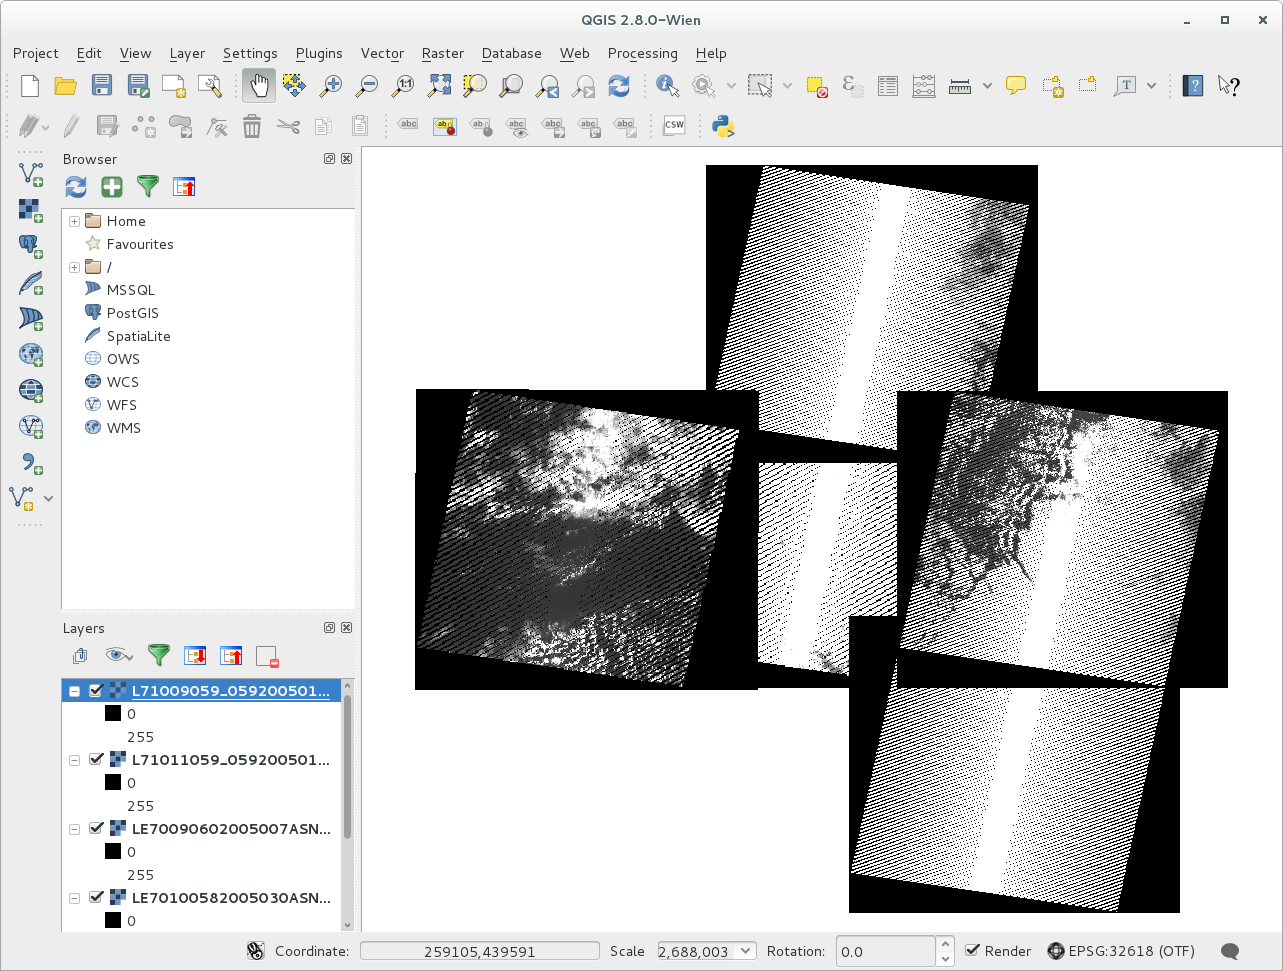
\includegraphics[width=12cm]{pictures/bio1.png}
  \caption{Imágenes Landsat de Nariño}
  \label{fig:bio1}
\end{figure}


\section{Reproyectar y recortar imágenes satelitales}

Debido a que las imágenes satelitales que cubren el departamento de Nariño, no estan en el mismo sistema de coordenadas, se tubo que hacer
una transformación de todas las imágenes a un mismo sistema de coordenadas, que además este sistema se pueda trabajar en metros decimales,
por lo tanto el sistema al cual se transformo fue al sistema EPSG:3857.

También debido a que las imágenes para el departamento de Nariño, sobrepasan mucho más el área del departamento, se recortó las imágenes
haciendo un buffer de 2500 metros de un shapfile del departamento y sobre este se extrajo el área del departamento, de esta manera los datos 
que se capturen únicamente corresponderan al departamento de Nariño, como lo muestra la figura~\ref{fig:bio2}

\begin{figure}[!htb]
  \centering
  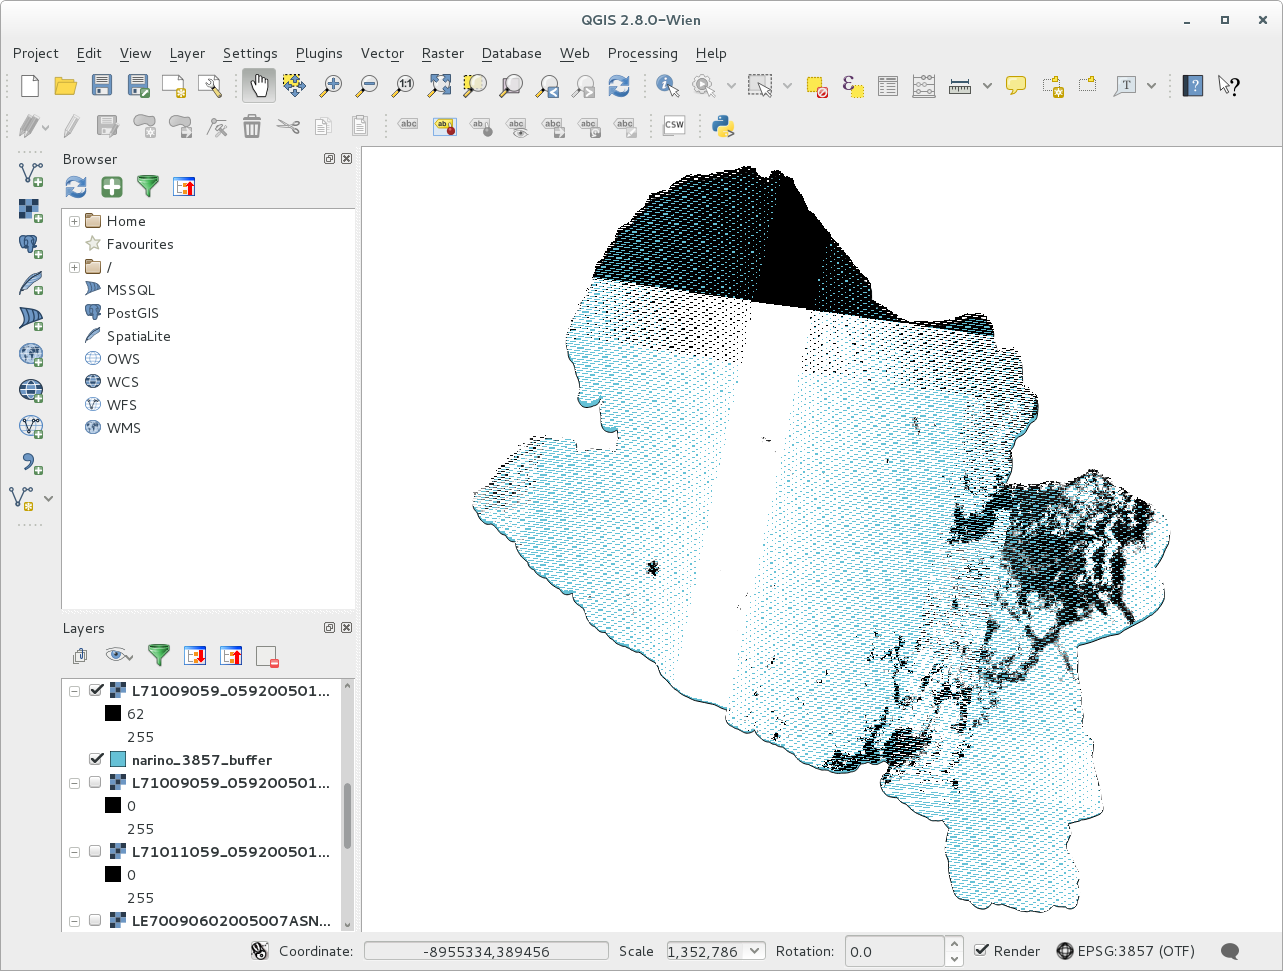
\includegraphics[width=12cm]{pictures/bio2.png}
  \caption{Imágenes Landsat de Nariño recortadas}
  \label{fig:bio2}
\end{figure}

Este proceso se aplico a las 1362 imágenes, para esto se lo realizo utilizando un script el cual se encuentra en repositorio del proyecto
\footnote{\url{https://github.com/poldrosky/alternar.git}}.


\section{Diseño de base de datos}

Se diseña una base de datos la cual va a guardar la información contenida en las imágenes satelitales, recorriendolas pixel a pixel. El diseño se lo puede mirar
en la figura~\ref{fig:dise}

\begin{figure}[!htb]
  \centering
  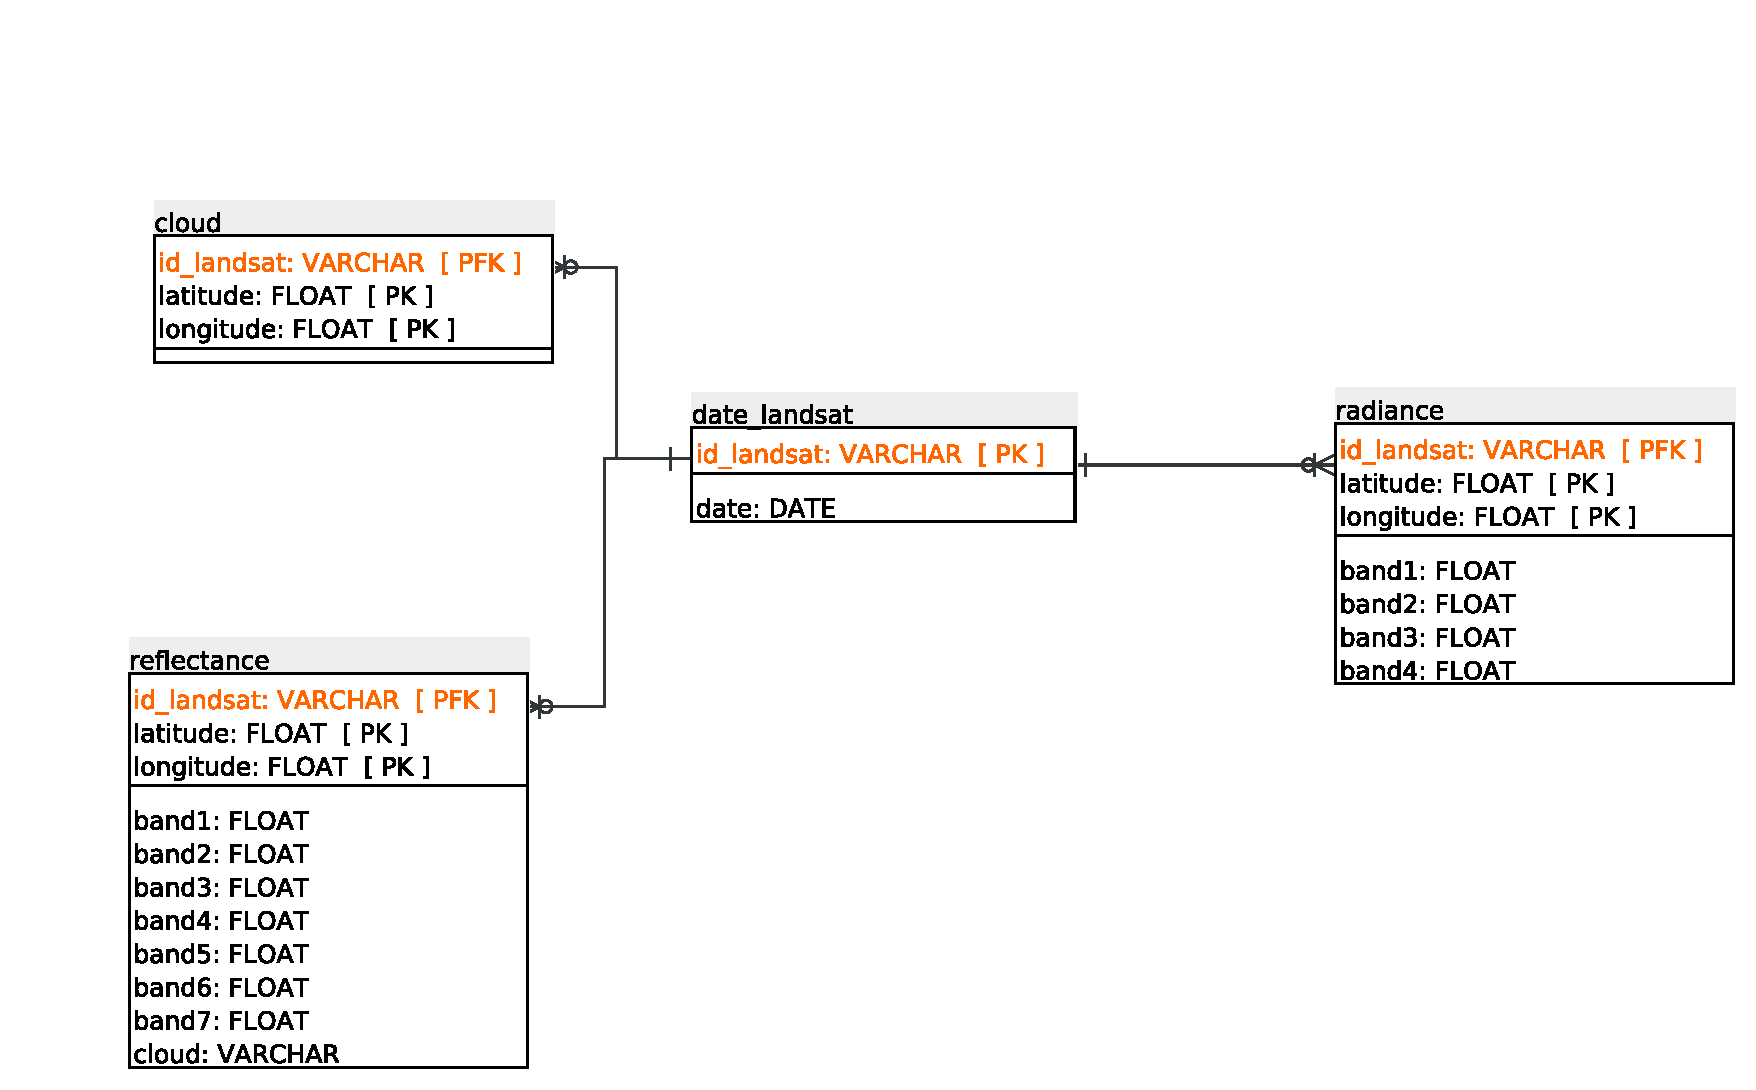
\includegraphics[width=12cm]{pictures/diagramaER.pdf}
  \caption{Diagrama ER de la Base de datos}
  \label{fig:dise}
\end{figure}


\section{Captura de información}

En la captura de información se tienen varios aspectos, como calculo de radiance, reflectance, y además se aplico un 
algoritmo propuesto en \cite{irish2000landsat}, en el cual se realiza un filtro para la detección de nubes.

Para la realización de este proceso se realizó un scrip que se encuentra en el repositorio del proyecto.




\bibliography{bibliography}
\bibliographystyle{IEEEtran}



\end{document}

